\documentclass[12pt,a4paper]{article}
\usepackage[utf8]{vietnam}
\usepackage{amsmath,amssymb}
\usepackage{geometry}
\geometry{top=1.5cm,bottom=1.2cm,left=1.4cm,right=1.4cm,headheight=28pt,headsep=12pt,footskip=18pt}
\usepackage{tikz}
\usepackage{xcolor}
\usepackage{enumerate}
\usepackage{graphicx}
\usepackage[version=4]{mhchem}
\usepackage{fancyhdr}
\usepackage{ex_test}

\renewcommand{\baselinestretch}{0.96}
\setlength{\parskip}{0pt}

\definecolor{hfRed}{RGB}{211,47,47}
\definecolor{hfGreen}{RGB}{139,195,144}

\providecommand{\False}{}

\pagestyle{fancy}
\fancyhf{}
\fancyhead[L]{\small\itshape\color{hfRed} Tài liệu lưu hành nội bộ}
\fancyhead[R]{\small\itshape\color{hfRed} Thầy \textbf{TRẦN VĂN THẠNH} - 0777.470.803}
\renewcommand{\headrulewidth}{0.8pt}
\renewcommand{\headrule}{\hbox to\headwidth{\color{hfGreen}\leaders\hrule height \headrulewidth\hfill}}

\fancyfoot[L]{\small\itshape\color{hfRed} CS1: 6/15 Nguyễn Hoàng, P. Kim Long, TP Huế \quad|\quad CS2: 24 Đặng Thái Thân, TP Huế}
\fancyfoot[R]{\small\bfseries\color{hfRed} Trang \thepage}
\renewcommand{\footrulewidth}{0.8pt}
\renewcommand{\footrule}{\hbox to\headwidth{\color{hfGreen}\leaders\hrule height \footrulewidth\hfill}}

\fancypagestyle{firstpage}{
  \fancyhf{}
  \renewcommand{\headrulewidth}{0pt}
  \fancyfoot[L]{\small\itshape\color{hfRed} CS1: 6/15 Nguyễn Hoàng, P. Kim Long, TP Huế \quad|\quad CS2: 24 Đặng Thái Thân, TP Huế}
  \fancyfoot[R]{\small\bfseries\color{hfRed} Trang \thepage}
  \renewcommand{\footrulewidth}{0.8pt}
  \renewcommand{\footrule}{\hbox to\headwidth{\color{hfGreen}\leaders\hrule height \footrulewidth\hfill}}
}

\begin{document}
\thispagestyle{firstpage}

\noindent
\begin{minipage}[t]{0.44\textwidth}
	\centering\fontsize{10pt}{12pt}\selectfont
	\textbf{SỞ GIÁO DỤC VÀ ĐÀO TẠO THỪA THIÊN HUẾ}\\
	\textbf{ĐỀ CHÍNH THỨC}\\
	\textit{(Đề thi có 04 trang)}
\end{minipage}\hfill
\begin{minipage}[t]{0.54\textwidth}
	\centering\small
	\textbf{ĐỀ KIỂM TRA ĐỊNH KỲ CHƯƠNG 1 (ESTER -- LIPID)}\\
	\textbf{MÔN: HOÁ HỌC -- LỚP 12}\\
	\textit{Thời gian làm bài: 50 phút (không kể thời gian phát đề)}\\
	\fbox{\textbf{MÃ ĐỀ: 102}}
\end{minipage}

\smallskip
\noindent\hrulefill
\smallskip

\noindent\textbf{Họ, tên thí sinh:} \dotfill\ \textbf{Lớp:} \dotfill\ \textbf{Số báo danh:} \dotfill

\smallskip
\noindent\textit{(Cho biết nguyên tử khối: H = 1; C = 12; N = 14; O = 16; Na = 23; K = 39; Br = 80; Cl = 35,5).}
\smallskip

\noindent
\textbf{PHẦN I (4,5 điểm -- 18 câu): Câu trắc nghiệm nhiều phương án lựa chọn.}\\
\textit{Thí sinh trả lời từ câu 1 đến câu 18. Mỗi câu hỏi thí sinh chỉ chọn một phương án.}

\Opensolutionfile{ans}[ans-de02hs]

\begin{ex}
$\ce{HCOOCH3}$ được sử dụng làm dung môi cho nitrocellulose và cellulose acetate, một chất trung gian trong sản xuất dược phẩm và thuốc xông hơi. Tên gọi của $\ce{HCOOCH3}$ là
\choice
{ethyl formate}
{ethyl acetate}
{methyl formate}
{methyl acetate}
\loigiai{}
\end{ex}

\begin{ex}
Ester nào sau đây tác dụng với $\ce{NaOH}$ thu được ethyl alcohol?
\choice
{$\ce{CH3COOC2H5}$}
{$\ce{CH3COOC3H7}$}
{$\ce{C2H5COOCH3}$}
{$\ce{HCOOCH3}$}
\loigiai{}
\end{ex}

\begin{ex}
Công thức tổng quát của ester mạch hở được tạo thành từ carboxylic acid no, đơn chức và alcohol no, đơn chức là
\choice
{$\ce{C_{n}H_{2n-1}COOC_{m}H_{2m+1}}$}
{$\ce{C_{n}H_{2n-1}COOC_{m}H_{2m-1}}$}
{$\ce{C_{n}H_{2n+1}COOC_{m}H_{2m-1}}$}
{$\ce{C_{n}H_{2n+1}COOC_{m}H_{2m+1}}$}
\loigiai{}
\end{ex}

\begin{ex}
Chất X có công thức cấu tạo $\ce{CH3CH2COOCH3}$ là một chất lỏng trong suốt với mùi trái cây và mùi thơm của rum. Tên gọi của X là
\choice
{propyl acetate}
{methyl propionate}
{methyl acetate}
{ethyl acetate}
\loigiai{}
\end{ex}

\begin{ex}
Thủy phân methyl propanoate trong môi trường acid thu được sản phẩm gồm:
\choice
{$\ce{CH3COOH}$ và $\ce{C3H7OH}$}
{$\ce{CH3COOH}$ và $\ce{C2H5OH}$}
{$\ce{C2H5COOH}$ và $\ce{C2H5OH}$}
{$\ce{C2H5COOH}$ và $\ce{CH3OH}$}
\loigiai{}
\end{ex}

\begin{ex}
Công thức nào sau đây có thể là công thức của chất béo?
\choice
{$\ce{CH3COOCH2C6H5}$}
{$\ce{C15H31COOCH3}$}
{$\ce{(C17H33COO)2C2H4}$}
{$\ce{(C17H35COO)3C3H5}$}
\loigiai{}
\end{ex}

\begin{ex}
Acid nào sau đây là acid béo?
\choice
{formic acid}
{oleic acid}
{acrylic acid}
{acetic acid}
\loigiai{}
\end{ex}

\begin{ex}
Chất không phải acid béo là
\choice
{acetic acid}
{palmitic acid}
{stearic acid}
{oleic acid}
\loigiai{}
\end{ex}

\begin{ex}
Hỗn hợp các muối sodium của acid béo sinh ra ở trạng thái keo. Để tách muối này ra khỏi hỗn hợp, người ta thêm chất gì vào hỗn hợp?
\choice
{tinh bột}
{muối ăn}
{nước}
{acid}
\loigiai{}
\end{ex}

\begin{ex}
Ester có công thức phân tử là $\ce{C2H4O2}$ được tạo thành từ methyl alcohol và carboxylic acid nào sau đây?
\choice
{propionic acid}
{acetic acid}
{formic acid}
{oxalic acid}
\loigiai{}
\end{ex}

\begin{ex}
Hợp chất nào dưới đây được sử dụng làm xà phòng?
\choice
{$\ce{CH3COONa}$}
{$\ce{CH3(CH2)14COONa}$}
{$\ce{CH3(CH2)12COOCH3}$}
{$\ce{CH3(CH2)5O(CH2)5CH3}$}
\loigiai{}
\end{ex}

\begin{ex}
Phản ứng xà phòng hóa là phản ứng xảy ra giữa
\choice
{chất béo với base}
{chất béo với sulfuric acid đặc}
{chất béo với acid béo}
{chất béo với acid hữu cơ}
\loigiai{}
\end{ex}

\begin{ex}
Chất nào cùng thành phần nguyên tố với chất béo?
\choice
{dầu mỏ}
{tinh dầu sả}
{ethylene}
{dầu bôi trơn}
\loigiai{}
\end{ex}

\begin{ex}
Nhận định nào sau đây đúng?
\choice
{Chất béo là triester của glycerol với acid béo}
{Xà phòng là muối của acid vô cơ}
{Mỡ động vật, dầu thực vật thường tan tốt trong nước}
{Dung dịch xà phòng có môi trường acid}
\loigiai{}
\end{ex}

\begin{ex}
Cho sơ đồ: $\ce{X + Y ->[t^\circ] \text{Xà phòng} + \text{glycerol}}$. Các chất X, Y có thể lần lượt là
\choice
{alcohol và base}
{ester và base}
{base và acid}
{ester và alcohol}
\loigiai{}
\end{ex}

\begin{ex}
Xét phân tử xà phòng có cấu tạo như hình bên:
\begin{center}
	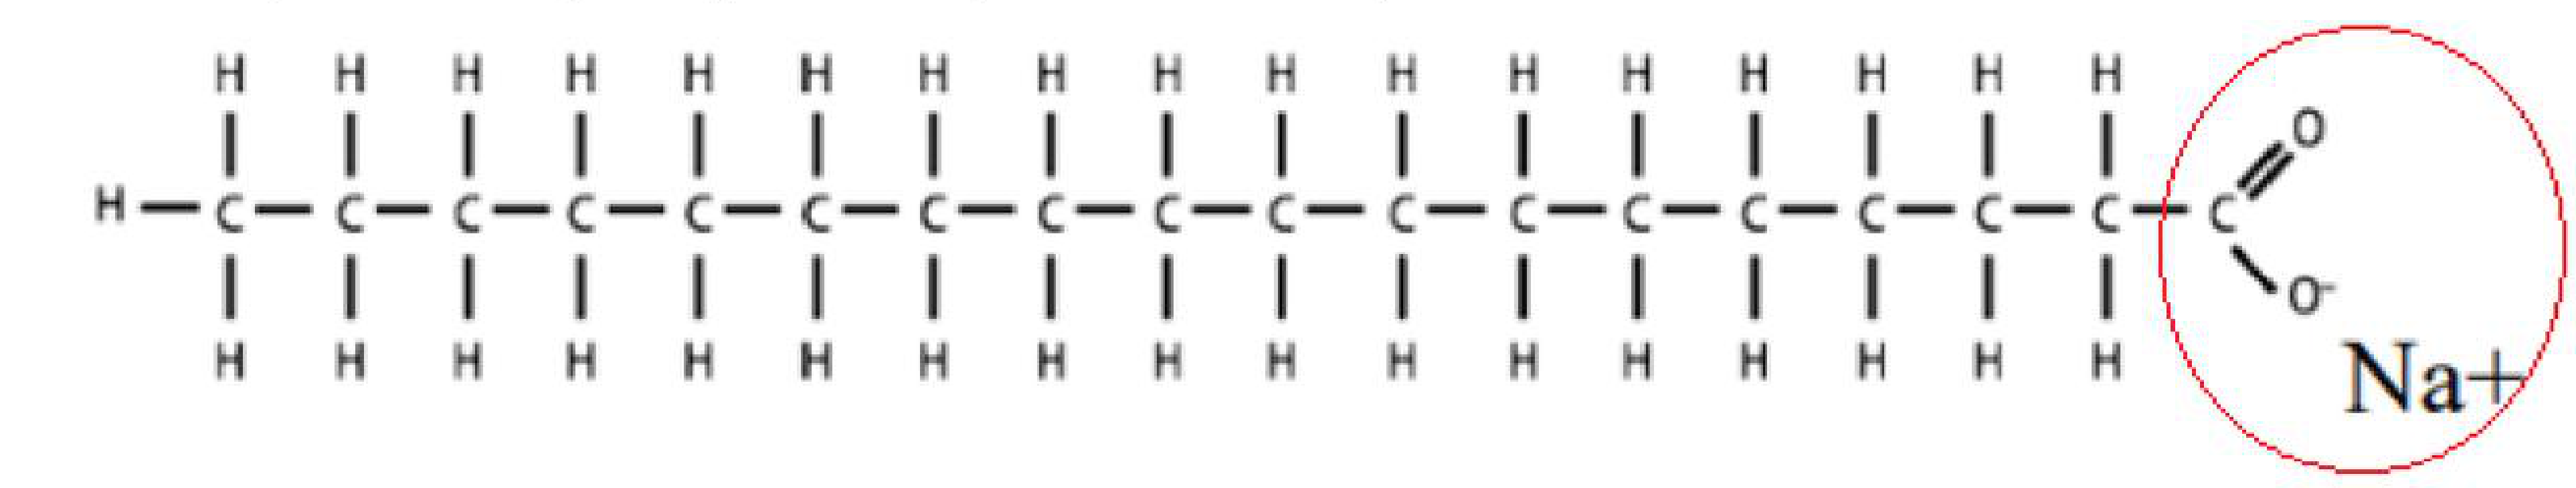
\includegraphics[width=13cm]{images_crop_de02/cau16_phan_tu_xa_phong.png}
\end{center}
Nhóm được khoanh tròn trong công thức trên là
\choice
{nhóm kị nước}
{nhóm dị thể}
{nhóm ưa nước}
{nhóm đồng thể}
\loigiai{}
\end{ex}

\begin{ex}
Thể tích $\ce{H2}$ (đkc) cần để hydrogen hóa hoàn toàn $1\text{ tấn}$ triolein là
\choice
{$84128{,}96\text{ L}$}
{$760{,}18\text{ lít}$}
{$7{,}6018\text{ lít}$}
{$7601{,}8\text{ lít}$}
\loigiai{}
\end{ex}

\begin{ex}
Cho $1\text{ mol}$ triglyceride X tác dụng với dung dịch $\ce{NaOH}$ dư, thu được $1\text{ mol}$ glycerol, $1\text{ mol}$ sodium palmitate và $2\text{ mol}$ sodium oleate. Phát biểu nào sau đây sai?
\choice
{Phân tử X có 5 liên kết $\pi$}
{Có 2 đồng phân cấu tạo thỏa mãn tính chất của X}
{Công thức phân tử chất X là $\ce{C52H96O6}$}
{$1\text{ mol}$ X làm mất màu tối đa $2\text{ mol}$ $\ce{Br2}$ trong dung dịch}
\loigiai{}
\end{ex}

\Closesolutionfile{ans}

\vspace{0.3cm}
\noindent
\textbf{PHẦN II (4,0 điểm -- 4 câu): Câu trắc nghiệm đúng sai.}\\
\textit{Thí sinh trả lời từ câu 1 đến câu 4. Trong mỗi ý a), b), c), d) ở mỗi câu, thí sinh chọn đúng hoặc sai.}

\setcounter{ex}{0}

\begin{ex}
Cho các phát biểu về acid béo và chất béo sau:
\choiceTF[t]
{Acid béo thường có gốc hydrocarbon mạch dài, có số nguyên tử carbon lẻ.}
{Khi xà phòng hoá chất béo, sản phẩm thu được là glycerol và các acid đơn chức.}
{Chất béo có nhiều gốc acid no thường ở dạng rắn, còn chất béo có nhiều gốc acid không no thường ở dạng lỏng.}
{Acid béo omega-3 là các acid béo không no có liên kết đôi đầu tiên ở vị trí số 3 nếu đánh số từ nhóm carboxyl (-COOH).}
\loigiai{}
\end{ex}

\begin{ex}
Người ta thực hiện phản ứng xà phòng hóa như hình vẽ dưới đây:
\begin{center}
	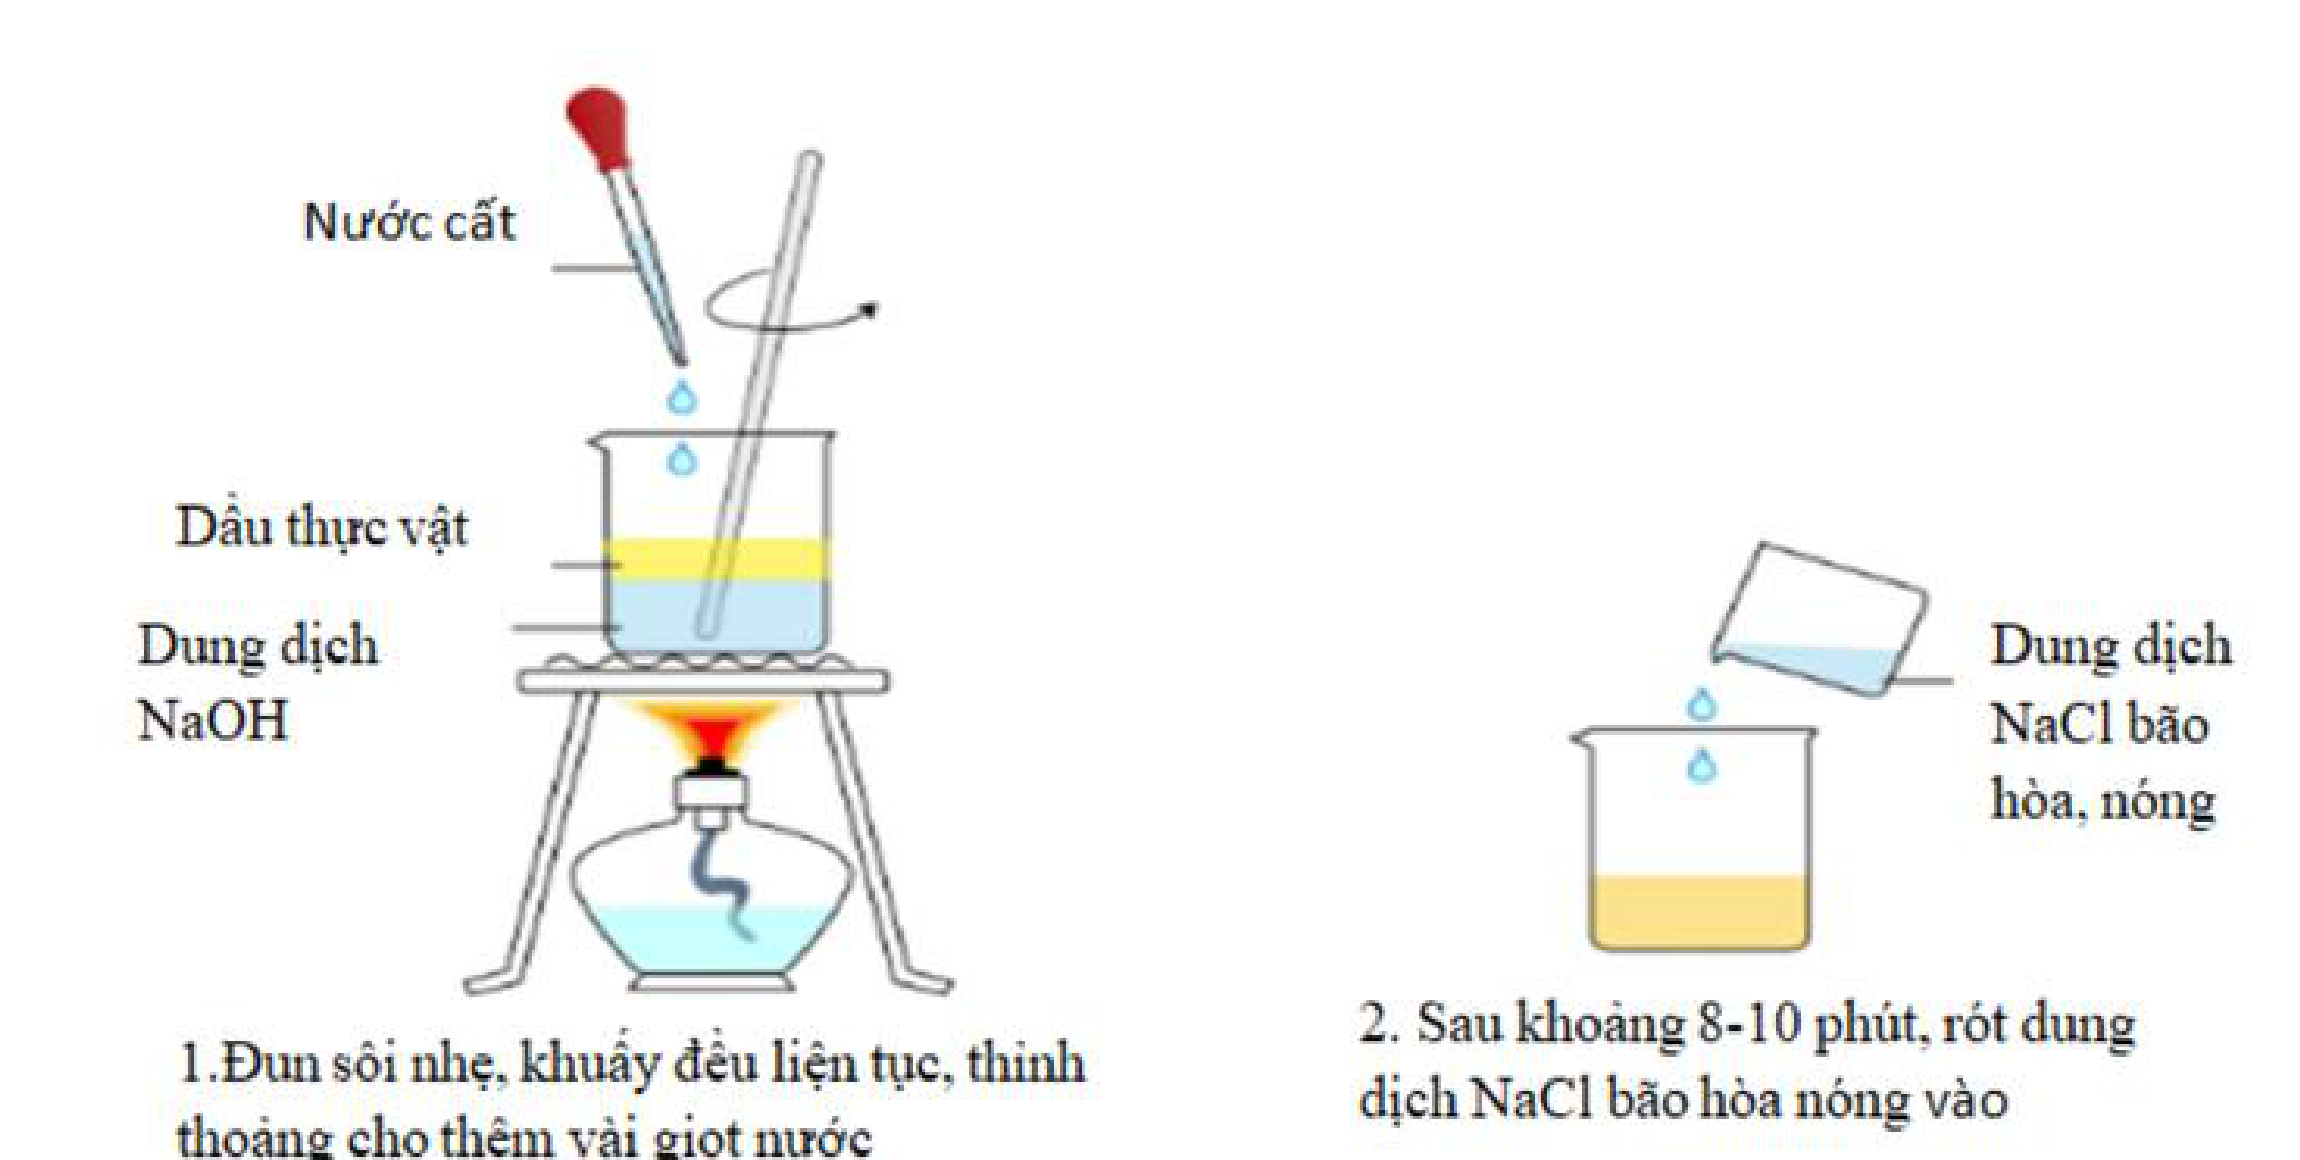
\includegraphics[width=9.5cm]{images_crop_de02/cau2_thi_nghiem_xa_phong_hoa.png}
\end{center}
Sau thí nghiệm, để nguội hỗn hợp trong cốc và quan sát:
\choiceTF[t]
{Khi đã nguội, hỗn hợp trong cốc tách thành 2 lớp.}
{Dung dịch $\ce{NaCl}$ bão hòa, nóng là xúc tác cho phản ứng xà phòng hóa.}
{Khi đã nguội, có một lớp glycerol nổi lên trên bề mặt hỗn hợp.}
{Phản ứng xảy ra trong thí nghiệm là phản ứng thủy phân ester trong môi trường kiềm.}
\loigiai{}
\end{ex}

\begin{ex}
Xét các phát biểu về xà phòng và chất giặt rửa:
\choiceTF[t]
{Chất kị nước là những chất không tan trong dầu mỡ, hydrocarbon,...}
{Muối sodium hoặc potassium của carboxylic acid được dùng làm xà phòng.}
{Xà phòng bị giảm hoặc mất tác dụng tẩy rửa khi dùng nước cứng vì gốc acid béo dễ kết tủa với cation $\ce{Ca^{2+}}, \ce{Mg^{2+}}$.}
{Xà phòng, chất giặt rửa tan vào nước tạo dung dịch có sức căng bề mặt nhỏ làm cho vật cần giặt rửa dễ thấm ướt.}
\loigiai{}
\end{ex}

\begin{ex}
Có bốn ống nghiệm: ống (1) chứa $3\text{ mL}$ nước cất; ống (2) chứa $3\text{ mL}$ nước xà phòng; ống (3) chứa $3\text{ mL}$ nước xà phòng và 3 giọt dung dịch $\ce{CaCl2}$ bão hoà; ống (4) chứa $3\text{ mL}$ nước giặt rửa tổng hợp và 3 giọt dung dịch $\ce{CaCl2}$ bão hoà. Cho vào mỗi ống nghiệm 3 giọt dầu ăn, lắc đều:
\choiceTF[t]
{Trong ống nghiệm (1), dầu ăn không tan và chìm xuống dưới.}
{Trong ống nghiệm (2), dầu ăn tan tạo hỗn hợp đồng nhất.}
{Trong ống nghiệm (3) có kết tủa xuất hiện.}
{Trong ống nghiệm (4), dầu ăn tan tạo hỗn hợp đồng nhất.}
\loigiai{}
\end{ex}

\vspace{0.3cm}
\noindent
\textbf{PHẦN III (1,5 điểm -- 6 câu): Câu trắc nghiệm yêu cầu trả lời ngắn.}\\
\textit{Thí sinh trả lời từ câu 1 đến câu 6. Mỗi câu hỏi thí sinh điền câu trả lời ngắn gọn theo yêu cầu.}

\setcounter{ex}{0}

\begin{ex}
Cho các chất sau: $\ce{C15H31COONa}$; $\ce{C15H31COOK}$; $\ce{CH3[CH2]11OSO3Na}$; $\ce{CH3[CH2]11C6H4SO3Na}$; $\ce{C17H33COOK}$. Số chất là thành phần chính của chất giặt rửa tổng hợp là bao nhiêu?
\loigiai{}
\end{ex}

\begin{ex}
Thuỷ phân hoàn toàn triglyceride X thu được glycerol và 3 acid béo là lauric acid, palmitic acid và oleic acid. X có thể có bao nhiêu công thức cấu tạo?
\loigiai{}
\end{ex}

\begin{ex}
Có bao nhiêu hợp chất hữu cơ đơn chức, phân tử chỉ chứa carbon, hydrogen, oxygen và có phân tử khối là 60?
\loigiai{}
\end{ex}

\begin{ex}
Chỉ số xà phòng hoá là số miligam $\ce{KOH}$ dùng để xà phòng hoá hết triglyceride và trung hoà hết lượng acid tự do trong $1\text{ g}$ chất béo. Một chất béo chứa 3,55\% stearic acid và 89\% tristearin về khối lượng, còn lại là các chất không tham gia phản ứng với $\ce{KOH}$. Tính chỉ số xà phòng hoá của chất béo trên.
\loigiai{}
\end{ex}

\begin{ex}
Xà phòng hoá hoàn toàn $0{,}1\text{ mol}$ ester E đơn chức, mạch hở bằng dung dịch $\ce{NaOH}$ vừa đủ thu được muối F và alcohol G. Biết khối lượng muối F thu được lớn hơn khối lượng ester E đã tham gia xà phòng hoá. Tính khối lượng alcohol G thu được (theo gam).
\loigiai{}
\end{ex}

\begin{ex}
Chỉ số xà phòng hóa (SAP): Lượng $\ce{KOH}$ cần thiết (tính bằng miligam) để phản ứng hết với $1\text{ gam}$ dầu, mỡ theo phản ứng xà phòng hóa và trung hòa hết carboxylic acid tự do có trong dầu, mỡ. Trong kĩ thuật, để tính lượng $\ce{NaOH}$ dùng để xà phòng hóa người ta xác định hệ số $a = \dfrac{\text{SAP}}{1402{,}5}$; $m_{\ce{NaOH}} = a \cdot m_{\text{chất béo}}\text{ (gam)}$. Biết loại dầu dừa có giá trị SAP là 255. Tính khối lượng của $\ce{NaOH}$ cần dùng để xà phòng hóa hết $200\text{ gam}$ dầu dừa. \textit{(Kết quả làm tròn đến hai chữ số thập phân)}.
\loigiai{}
\end{ex}


\begin{center}
	\textbf{---------- HẾT ----------}
\end{center}

\end{document}
